\section{System Overview}
FE.ED is an automatic pet feeder that is designed to work for up to two pets. The system consists of the automatic pet feeder, which is able to store and dispense dry pet food, the web application to facilitate user interaction with the robot and a flask server that connects the web app to the robot.

This user guide will outline steps on how to setup the robot, the app and server as well as covering typical uses of the robot. A troubleshooting table is also provided at the end of this guide.



    \subsection{System Components and Prerequisites}
       To follow the steps throughout this guide, you will need the following:
       \begin{itemize}
           \item The robot - this includes the smart bowls outlined later in the guide
           \item Any necessary files which are discussed in this guide. Links will be provided for any necessary files.
           \item A computer with internet connection
       \end{itemize}
    \subsection{Robotic Guide}
    
        \subsubsection{Mechanical Structure}
        The images below outlines the structure of the robot as well as the key components:
        \begin{figure}[h]
        \centering
        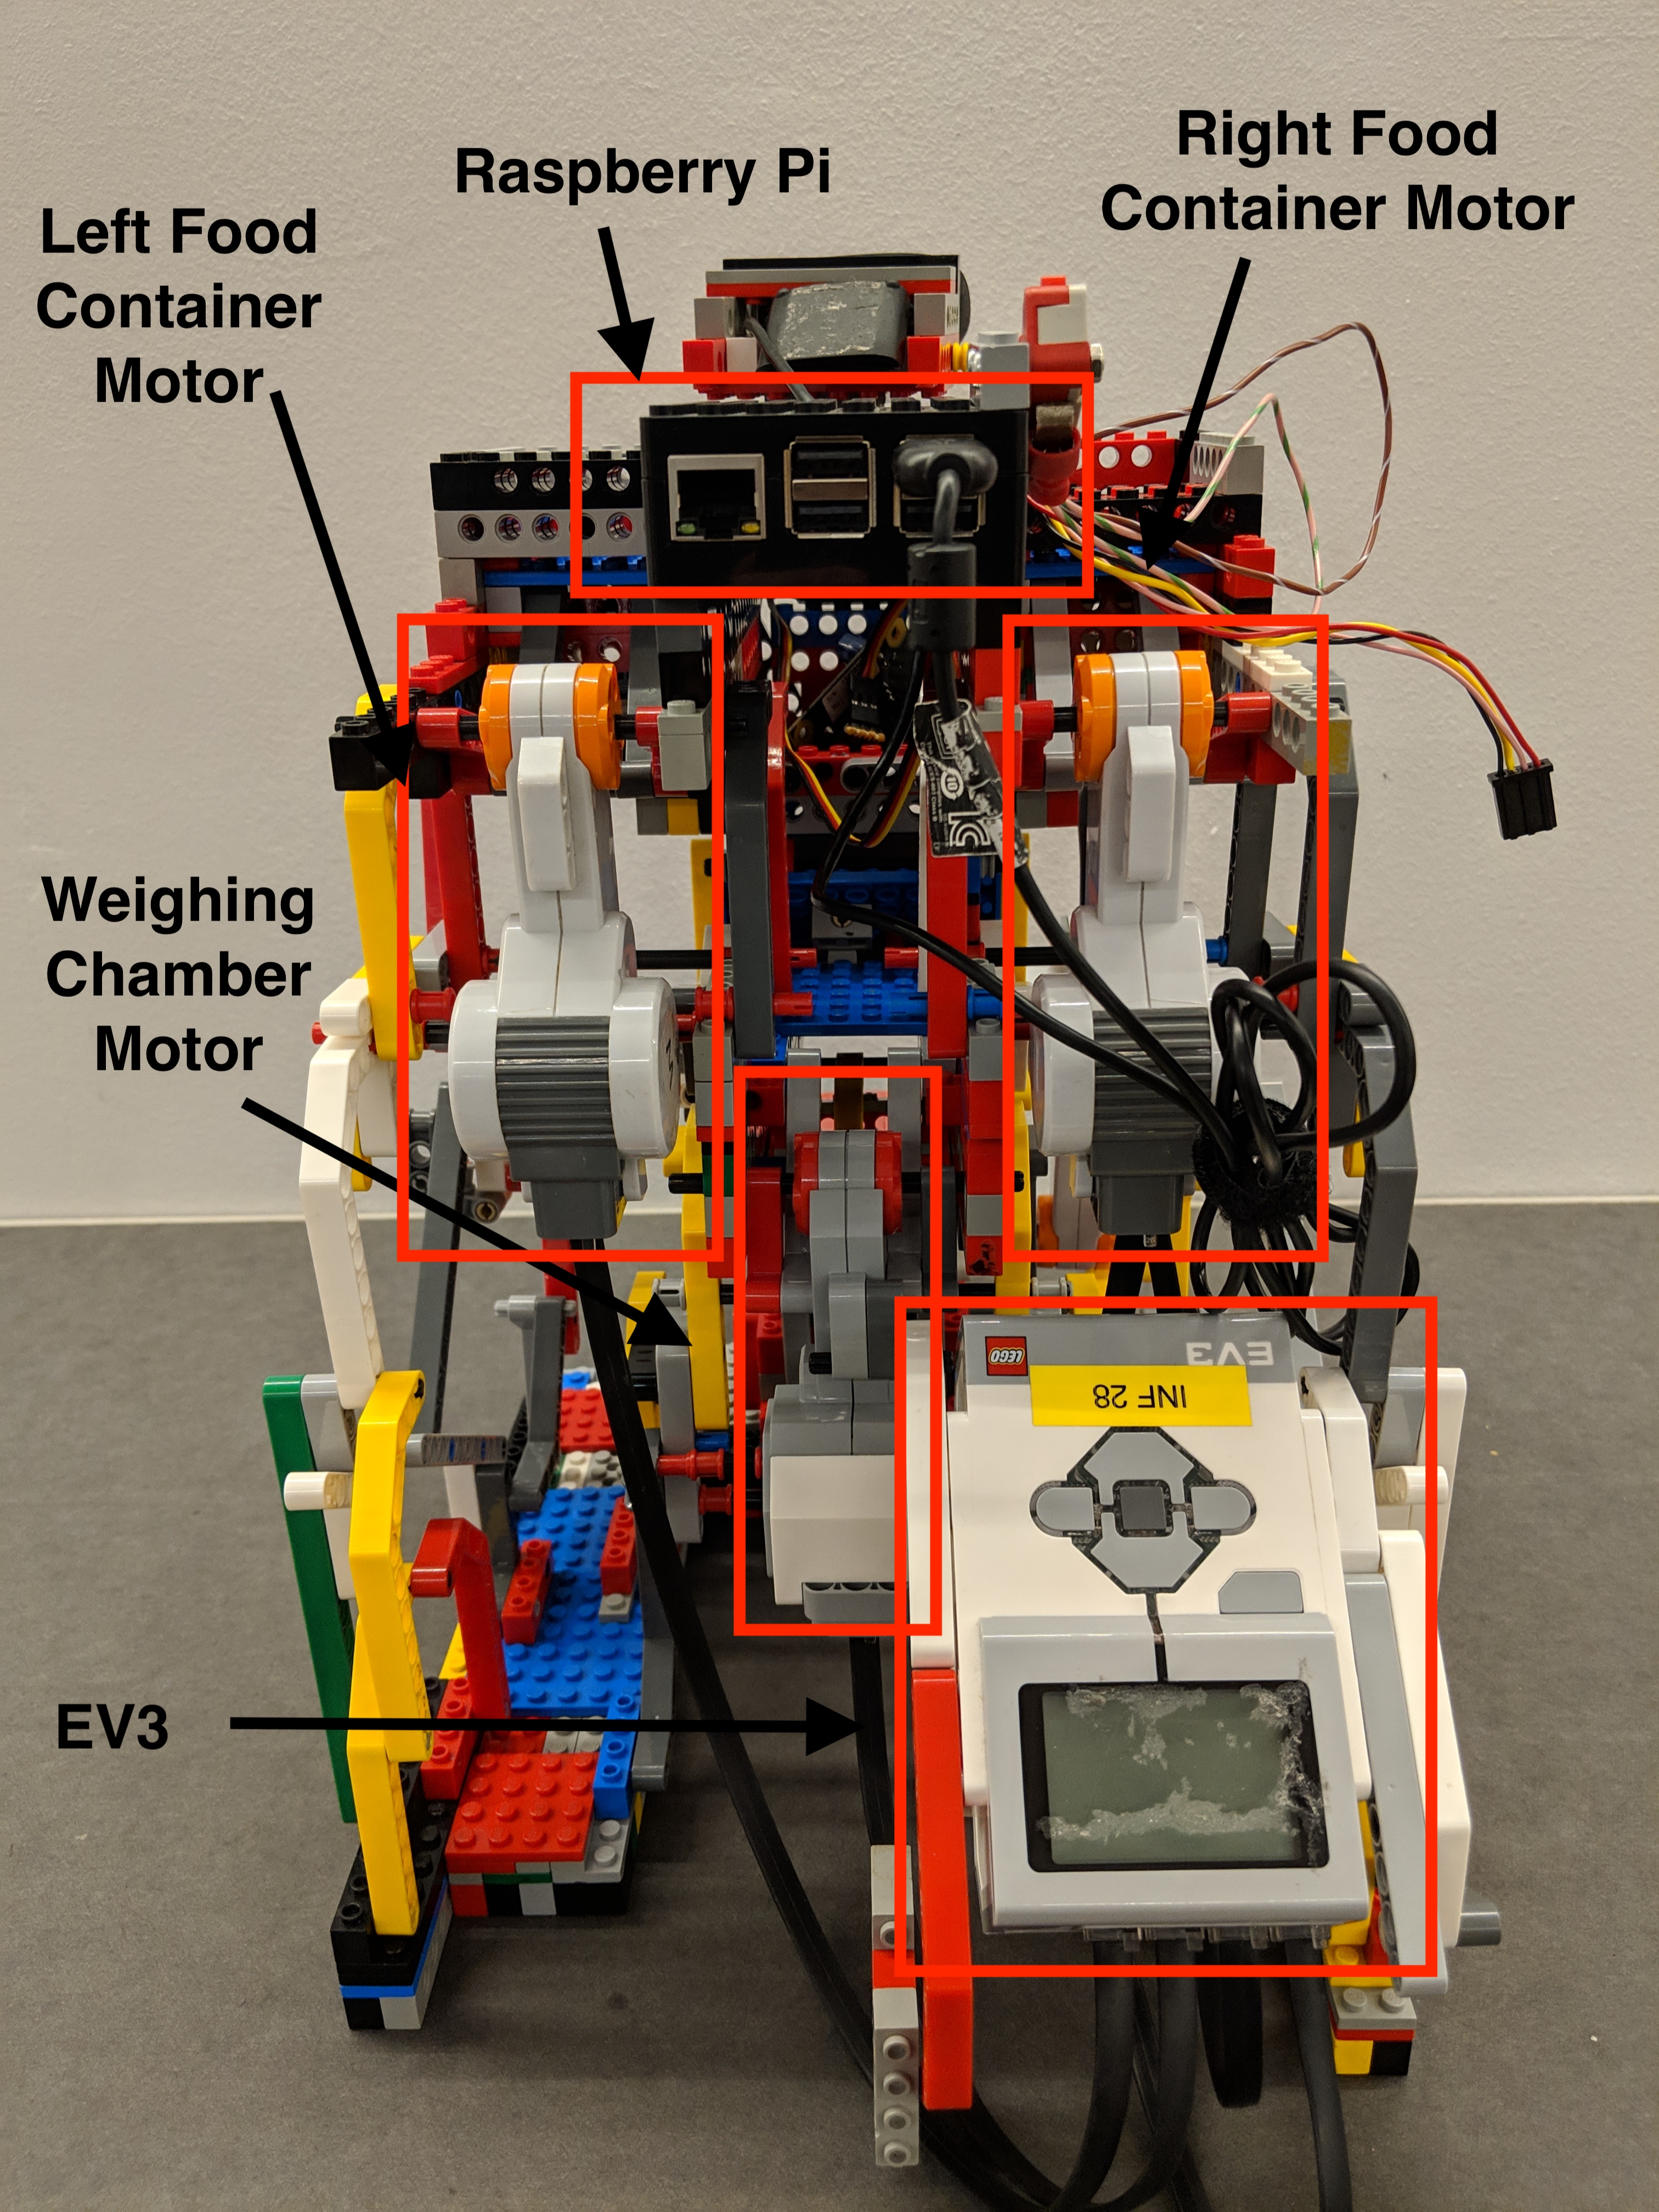
\includegraphics[width=8cm]{back_rob.jpg}
         \caption{Back of the robot}
        \end{figure}
        
        \newpage
        
        \begin{figure}[h]
        \centering
        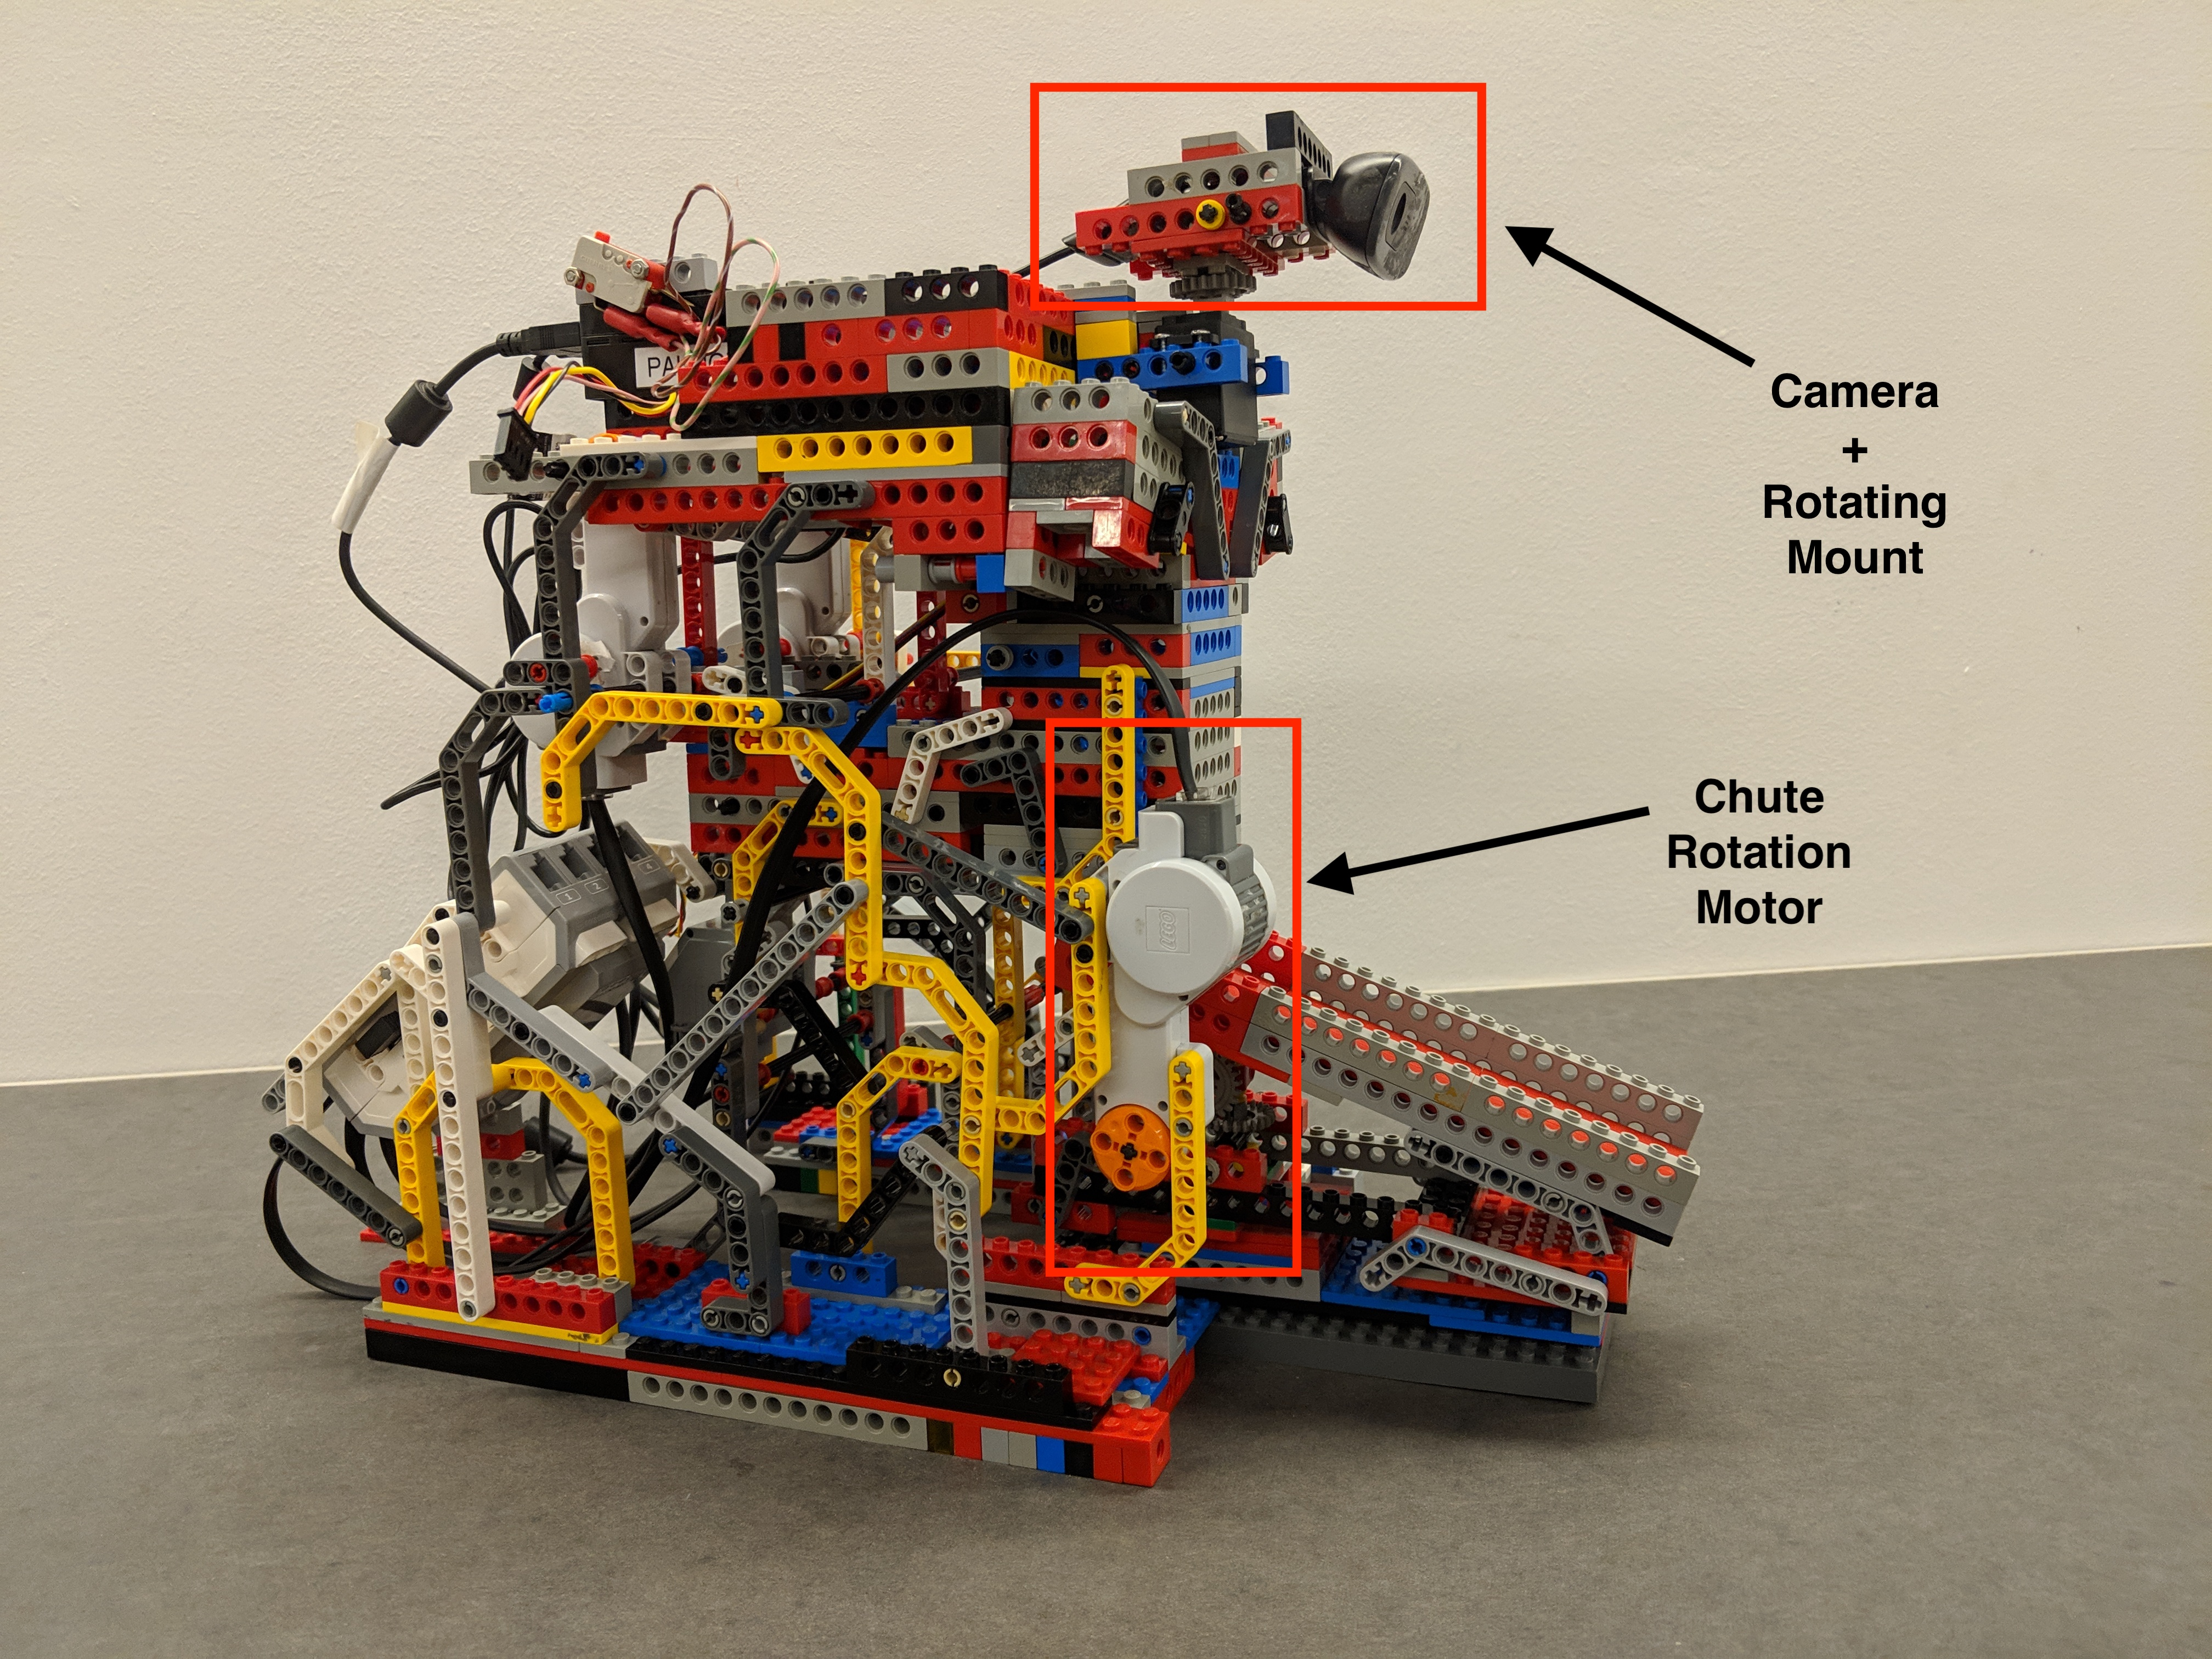
\includegraphics[width=8cm]{Side_rob.jpg}
         \caption{Side of the robot}
        \end{figure}
        
        The pet feeder is powered by four different EV3 motors, as well as the Raspberry Pi. The EV3 motors are responsible for dispensing the desired quantity of food into the specified bowl. The food is dispensed through a sliding trap door mechanism to ensure a continuous and controlled flow of food. 
        
        The camera is located on top of a rotating mount, powered by a servo motor, that is connected to the Raspberry Pi. This allows a smooth and responsive rotation. There are built in weight sensors in the bowls as well as the weighing chamber to give accurate and up to date readings. The weight sensors in the smart bowls allow for accurate readings on the current weight of the bowls, this is transmitted back to the server. The weight sensors are connected to the Arduino which is connected via USB to the Raspberry Pi.
        
        \begin{figure}[h]
        \centering
        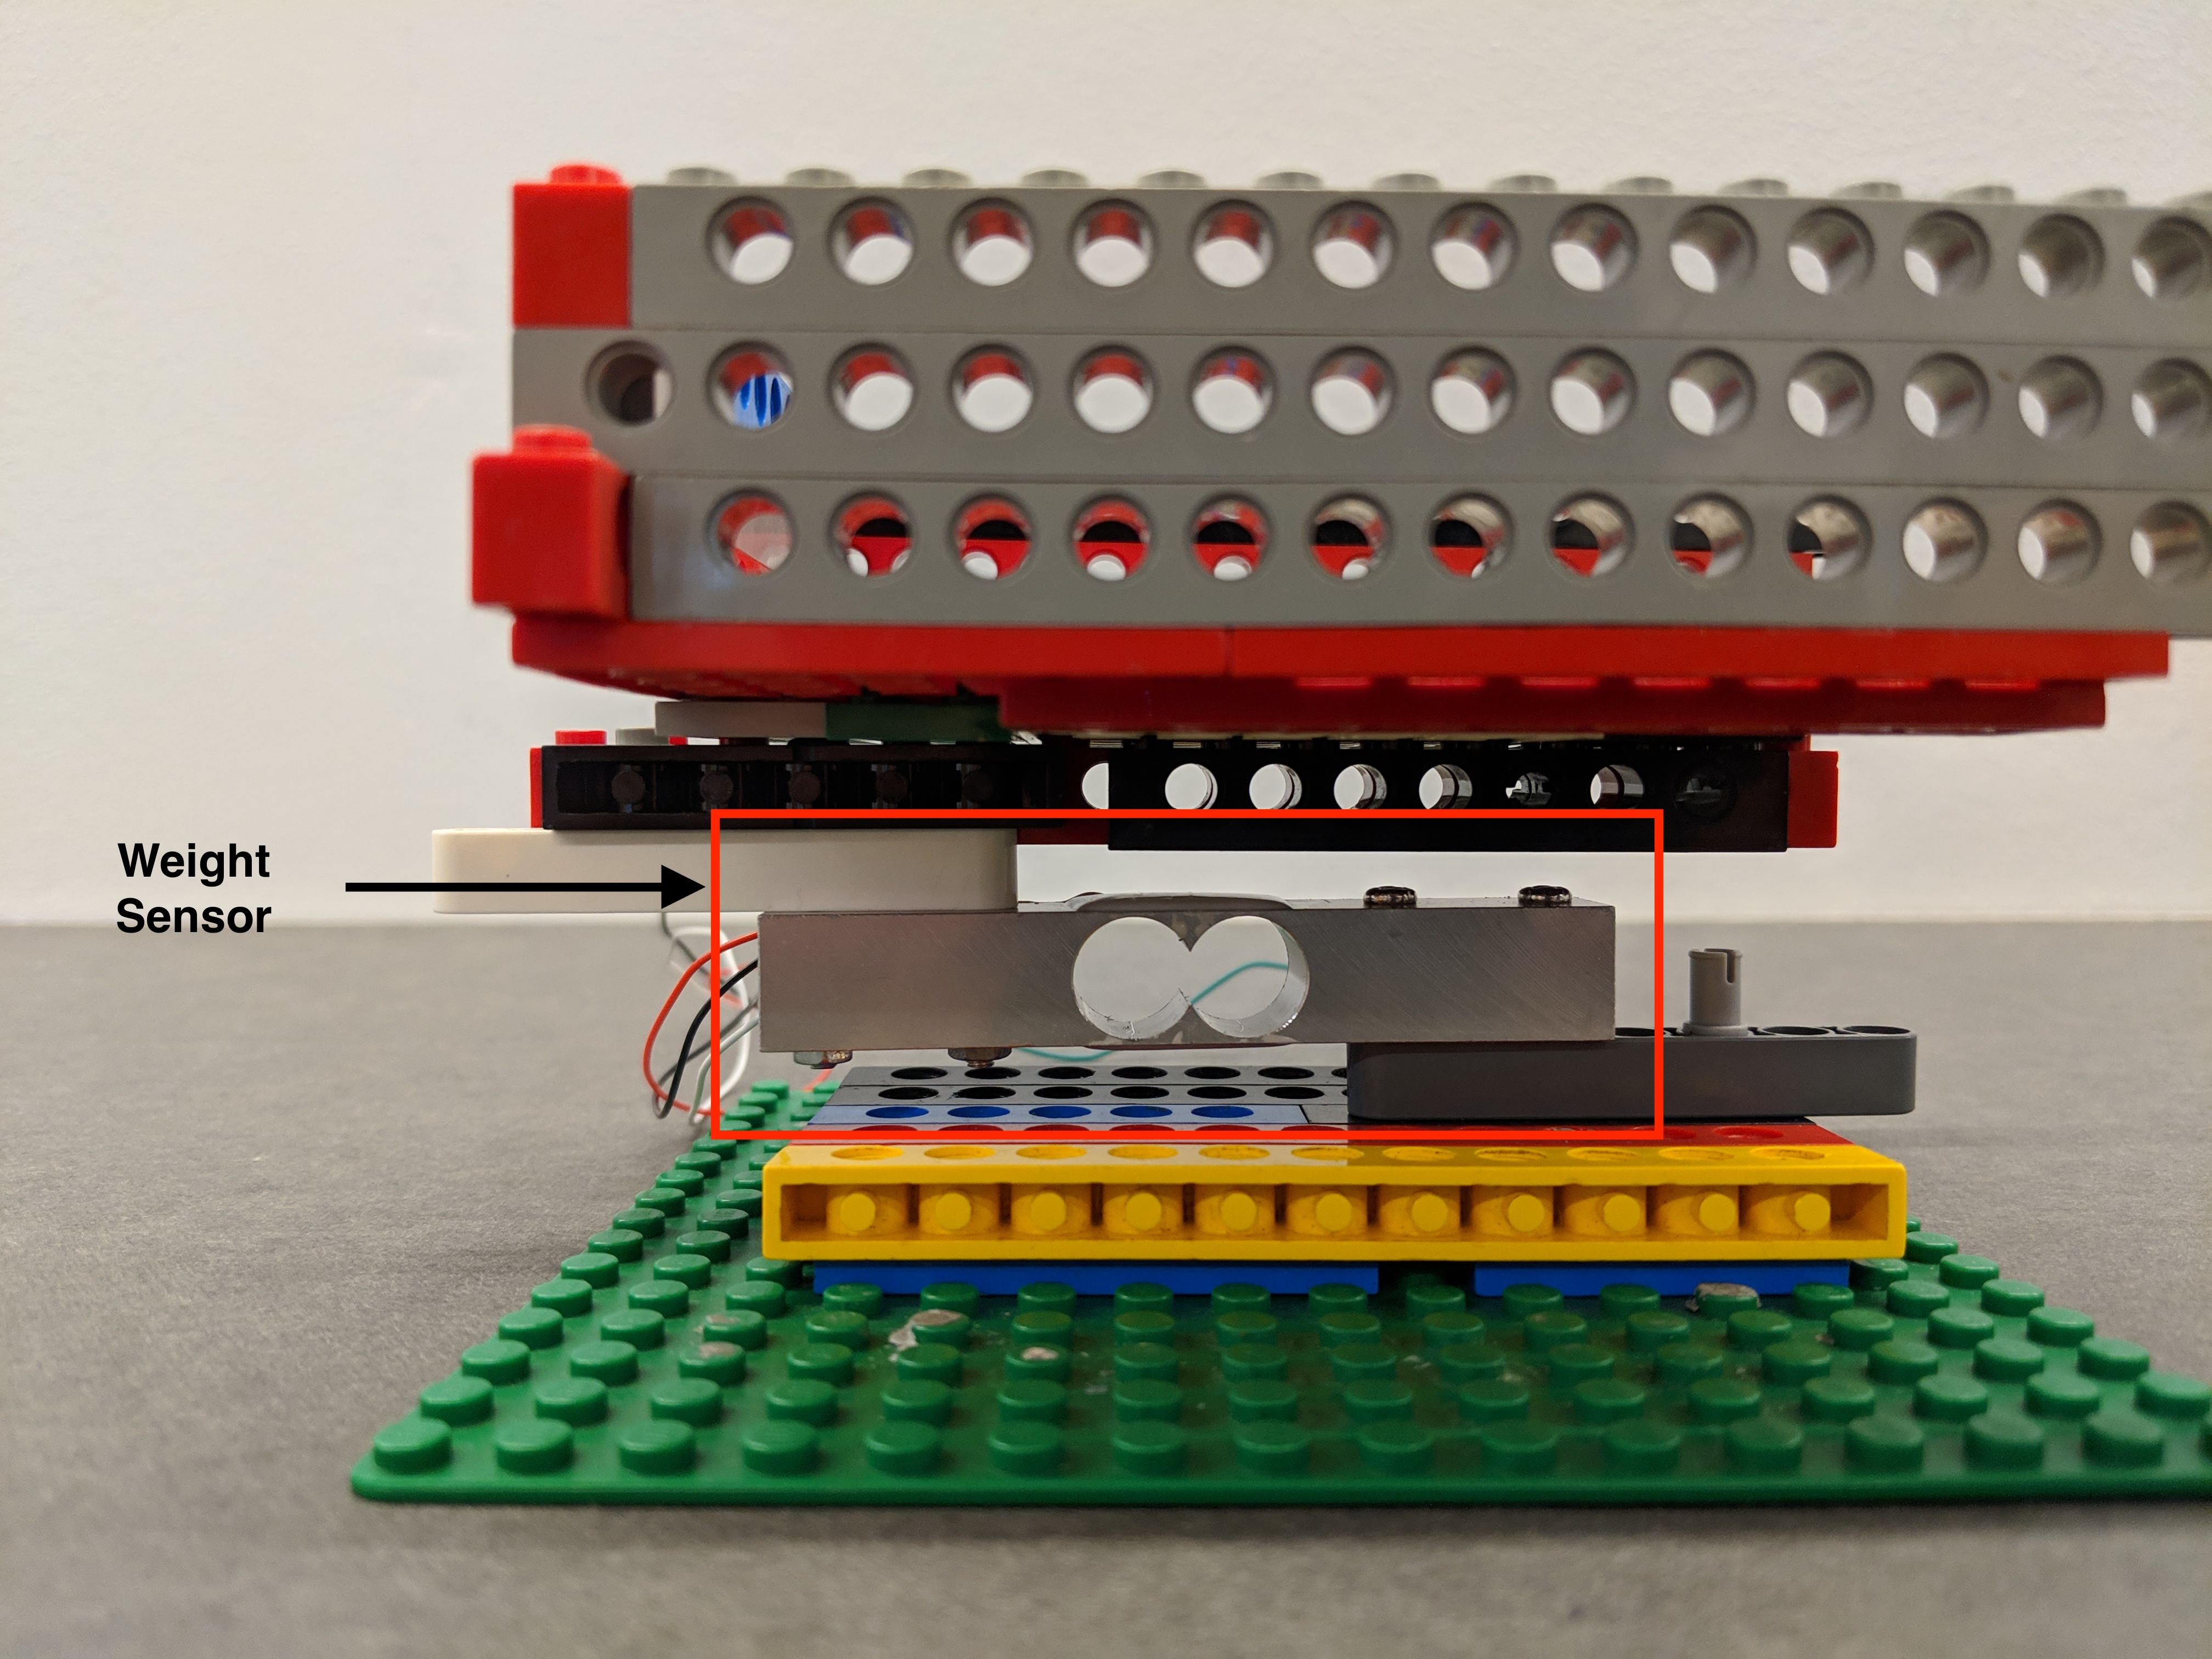
\includegraphics[width=6cm]{weightSensor.jpg}
         \caption{Weight Sensor}
        \end{figure}
        
         \begin{figure}[h]
        \centering
        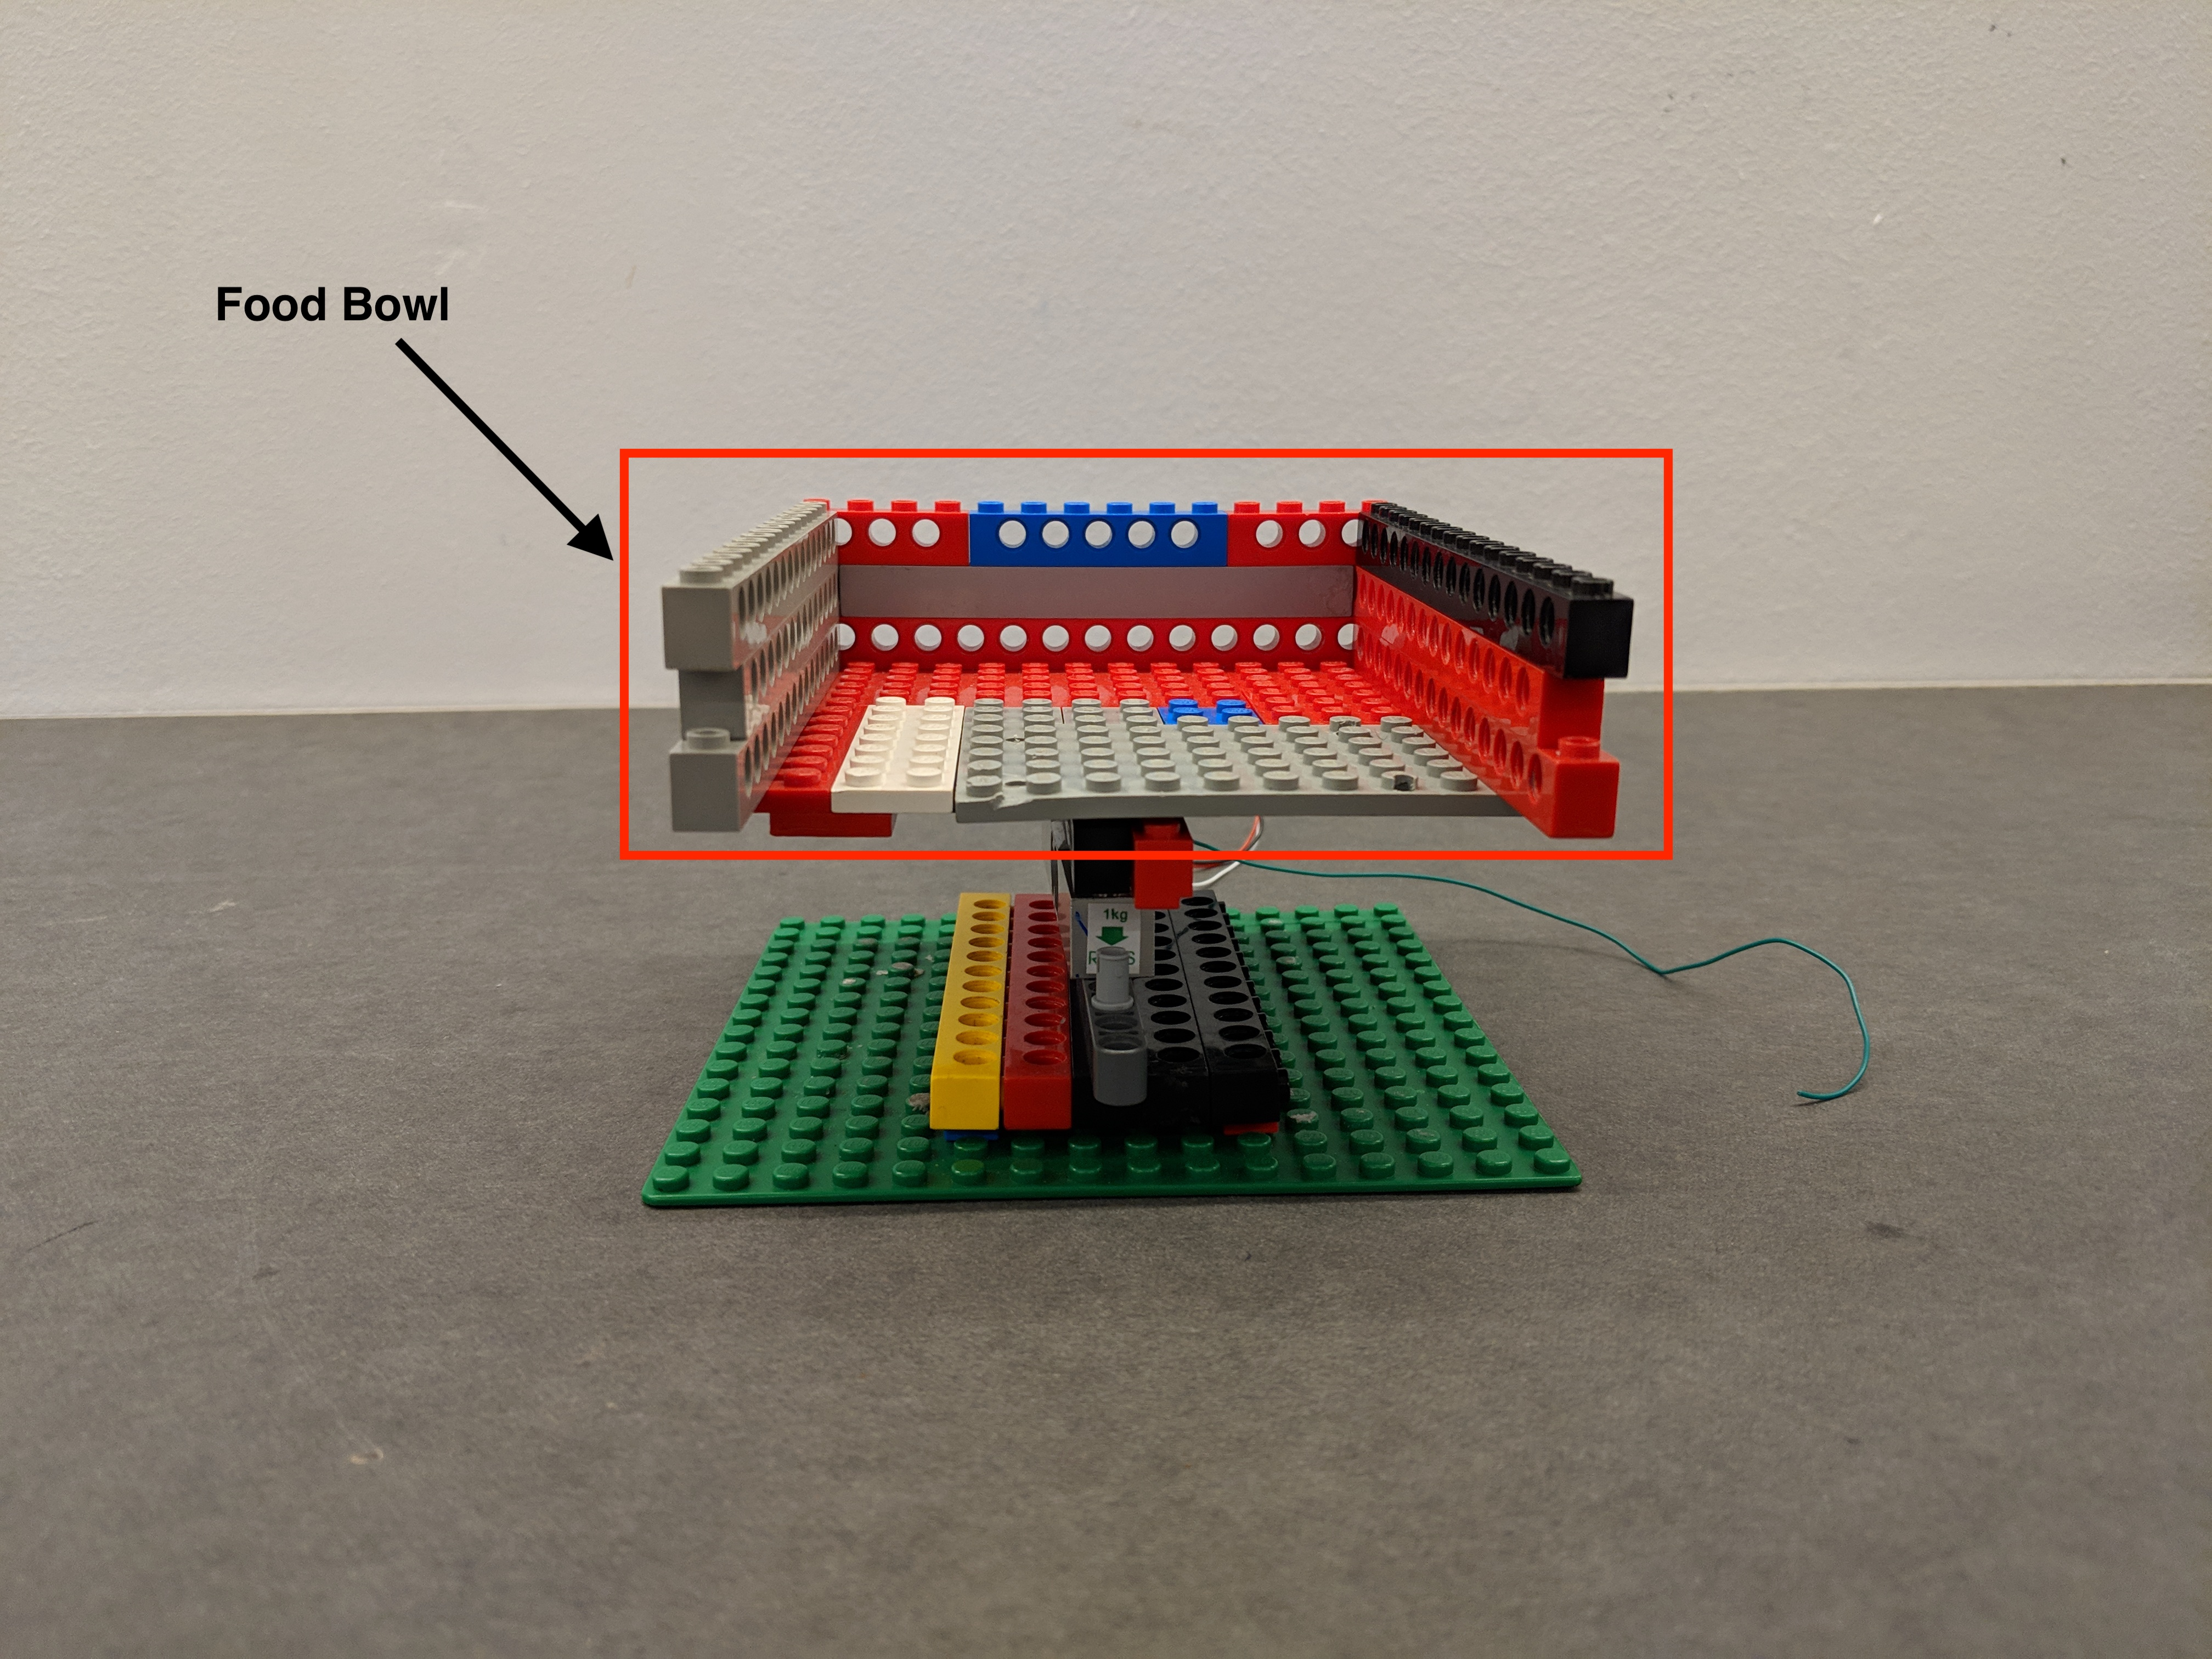
\includegraphics[width=6cm]{foodBowl.jpg}
         \caption{Food Bowl}
        \end{figure}
        

        \subsubsection{Component Location and Connection}
        Table 1 shows where components are connected
        
        \begin{table}[h!]
            \centering
             \begin{tabular}{||c | c||} 
             \hline \hline
             Component & Connection \\ [0.5ex] 
             \hline\hline
             Left Food Container Motor & EV3 Port D  \\ [1ex] \hline 
             Right Food Container Motor & EV3 Port C  \\ [1ex] \hline 
             Weighing Chamber Motor & EV3 Port B \\ [1ex] \hline 
             Chute Rotating Motor & EV3 Port A  \\ [1ex]  \hline 
             Camera Rotating Motor & Raspberry Pi  \\ [1ex] \hline 
             Camera & Raspberry Pi \\ [1ex] \hline 
             Arduino Board & Raspberry Pi \\ [1ex] \hline 
             \hline 
             \end{tabular}
             \caption{Component Connections}
        \end{table}
        
    
        
    \subsection{Software Structure}
    
    The three main components of FE.ED include:
    \begin{itemize}
        \item \textbf{Robot}: Stores the pet food in containers and dispenses the food at the scheduled time 
        \item \textbf{Web Application}: Responsible for allowing the user to interact with the robot through a graphical interface
        \item \textbf{Server}: Allows communication between the raspberry pi and the web application
    \end{itemize}
    
      \begin{figure}[h]
        \centering
        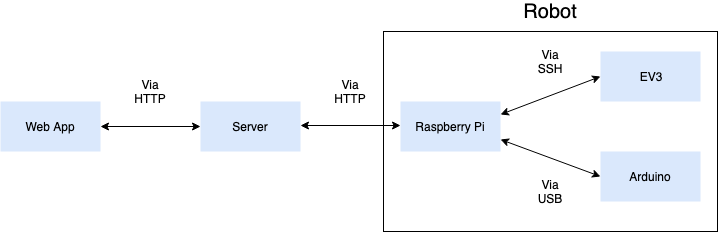
\includegraphics[width=\textwidth]{structure.png}
         \caption{Structure of the Software System}
        \end{figure}
    
